% 2020 北京卷 第 16 题：正方体 ABCD-A1B1C1D1，E 为 BB1 的中点
% 来源 PDF：普通高考/2020/2020北京.pdf 第 1 页（A3 横排），印面 1113，第 16 题右侧
% 重绘依据：原页该图为矢量路径，pdftocairo -svg 解出全部端点后按棱长归一化逐个还原。
%   原页画法：前侧面为正方形 D1C1CD（D 在左下、C 在右下、C1 在右上、D1 在左上），
%   深度方向朝右上（斜二测，长度约为棱长的一半）；后侧面 A1B1BA 与前侧面平行，
%   A 是被遮挡的顶点，故 AA1、AB、AD、AD1、AE 画虚线，D1E 亦为虚线；
%   E 位于 BB1 的中点。
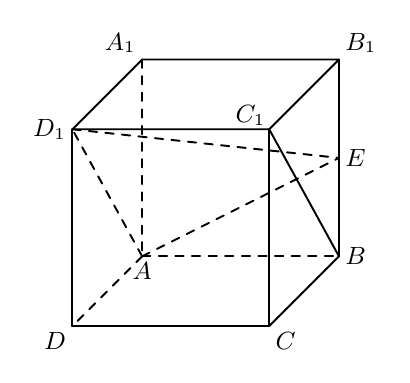
\begin{tikzpicture}[line width=0.7pt, font=\small,
  x=1.25cm, y=1.25cm, line cap=round, line join=round]

  % 顶点坐标（棱长 2，深度偏移 (0.709, 0.709)）
  \coordinate (D)  at (0.000, 0.000);
  \coordinate (C)  at (2.000, 0.000);
  \coordinate (C1) at (2.000, 2.000);
  \coordinate (D1) at (0.000, 2.000);
  \coordinate (A)  at (0.709, 0.709);
  \coordinate (B)  at (2.709, 0.709);
  \coordinate (B1) at (2.709, 2.709);
  \coordinate (A1) at (0.709, 2.709);
  \coordinate (E)  at (2.709, 1.709);

  % 上底面四边（实线）
  \draw (A1) -- (B1) -- (C1) -- (D1) -- cycle;

  % 可见棱（实线）
  \draw (D1) -- (D);
  \draw (C1) -- (C);
  \draw (D) -- (C);
  \draw (B1) -- (B);
  \draw (B) -- (C);
  \draw (B) -- (C1);

  % 被遮挡的棱与体内连线（虚线）
  \draw[dashed] (A1) -- (A);
  \draw[dashed] (A) -- (B);
  \draw[dashed] (A) -- (D);
  \draw[dashed] (A) -- (D1);
  \draw[dashed] (A) -- (E);
  \draw[dashed] (D1) -- (E);

  % 顶点标注
  \node[above left, inner sep=2pt]  at (A1) {$A_1$};
  \node[above right, inner sep=2pt] at (B1) {$B_1$};
  \node[above left, inner sep=1pt]  at (C1) {$C_1$};
  \node[left, inner sep=2pt]        at (D1) {$D_1$};
  \node[below, inner sep=2pt]       at (A)  {$A$};
  \node[right, inner sep=2pt]       at (B)  {$B$};
  \node[below right, inner sep=2pt] at (C)  {$C$};
  \node[below left, inner sep=2pt]  at (D)  {$D$};
  \node[right, inner sep=2pt]       at (E)  {$E$};
\end{tikzpicture}
